
\section{World Bank}
\label{sec-1}







    
  
  
\subsection{The Phillips curve}
\label{sec-1-1}



Instead of using different panels for each country, comparisons
are easier if the collection of country curves is superposed in
one panel. Each curve will be distinguished with its color and
label.
\subsection{Choosing colors}
\label{sec-1-2}


The \texttt{Country.Name} categorical variable will be encoded with a
qualitative palette, for example the \texttt{Set1} palette of the
\texttt{RColorBrewer}. Since this palette provides only 9 colors we have
to repeat some colors to complete the number of levels of the
variable \texttt{Country.Name}. The result is a palette with non-unique
colors, and thus some countries will share the same color. This is
not a problem since the curves will be labelled, and countries with
the same color will be displayed at enough distance.
\index{Packages!RColorBrewer@\texttt{RColorBrewer}}
\index{brewer.pal@\texttt{brewer.pal}}

\lstset{language=R}
\begin{lstlisting}
library(RColorBrewer)

nCountries <- nlevels(CO2data$Country.Name)
pal <- rep(brewer.pal(n=9, 'Set1'),
           length = nCountries)
\end{lstlisting}

Adjacent colors of this palette are easily
distinguishable. Therefore, the connection between colors and
countries must be in a such a way that nearby lines are encoded
with adjacent colors of the palette. 

A simple approach is to calculate the annual average of the
variable to be represented along the x-axis (\texttt{CO2.capita}), and
extract colors from the palette according to the order of this
value.  
\index{aggregate@\texttt{aggregate}}

\lstset{language=R}
\begin{lstlisting}
## Rank of average values of CO2 per capita
CO2mean <- aggregate(CO2.capita ~ Country.Name, data=CO2data, FUN=mean)
palOrdered <- pal[rank(CO2mean$CO2.capita)]
\end{lstlisting}

A more sophisticated solution is to use the ordered results of a
hierarchical clustering of the time evolution of the $CO_2$ per
capita values. The data is extracted from the original CO2
\texttt{data.frame}.  
\index{hclust@\texttt{hclust}}

\lstset{language=R}
\begin{lstlisting}
CO2capita <- subset(CO2, Indicator.Code=='EN.ATM.CO2E.PC')
hCO2 <- hclust(dist(CO2capita[, -c(1:4)]))
\end{lstlisting}


\lstset{language=R}
\begin{lstlisting}
plot(hCO2, labels=CO2capita$Country.Name,
     xlab='', ylab='', sub='', main='')
\end{lstlisting}

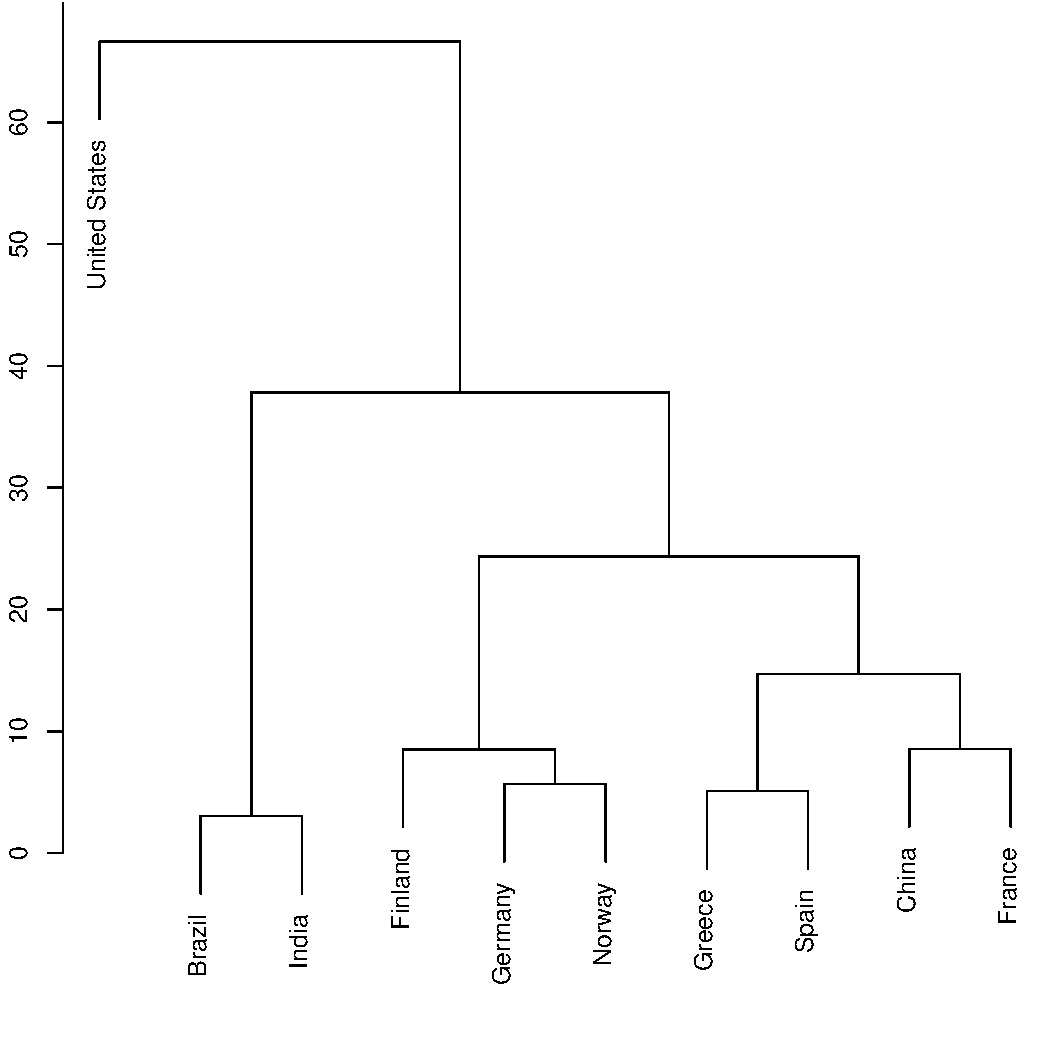
\includegraphics[width=.9\linewidth]{figs/hclust.pdf}

The colors of the palette are assigned to each country with \texttt{match},
which returns a vector of the positions of the matches of
\texttt{levels(CO2data\$Country.Name)} (country names in alphabetical order)
in \texttt{CO2capita\$Country.Name[hCO2\$order]} (country names ordered
according to the hierarchical clustering). 

\lstset{language=R}
\begin{lstlisting}
idx <- match(levels(CO2data$Country.Name), 
             CO2capita$Country.Name[hCO2$order])
palOrdered <- pal[idx]
\end{lstlisting}

Finally, with \texttt{custom.theme}, the palette is encapsulated in a new
theme for \texttt{xyplot}. It must be highlighted that this palette links
colors with the levels of \texttt{Country.Name} (country names in
alphabetical order), which is exactly what the \texttt{groups} argument
provides.  

\index{custom.theme@\texttt{custom.theme}}

\lstset{language=R}
\begin{lstlisting}
myTheme <- custom.theme(pch=19, cex=0.6, symbol=palOrdered)

pCO2.capita <- xyplot(GNI.capita  ~ CO2.capita,
                      xlab="CO2 emissions (metric tons per capita)",
                      ylab="GNI per capita, PPP (current international $)",
                      groups=Country.Name, data=CO2data,
                      par.settings=myTheme,
                      type='b')
\end{lstlisting}

This \texttt{trellis} object displays a curve for each country using
different colors to distinguish them. A first improvement is to show
the time evolution with labels displaying the years.  A panel function
with \texttt{panel.text} to print the year labels, and \texttt{panel.superpose} to
display the lines for each group will do the work. In the panel
function, \texttt{subscripts} is a vector with the integer indices
representing the rows of the \texttt{data.frame} to be displayed in the
panel.


\index{panel.text@\texttt{panel.text}}
\index{subscripts@\texttt{subscripts}} \index{Panel function}
\index{panel.superpose@\texttt{panel.superpose}}

\lstset{language=R}
\begin{lstlisting}
xyplot(GNI.capita  ~ CO2.capita,
       xlab="CO2 emissions (metric tons per capita)",
       ylab="GNI per capita, PPP (current international $)",
       groups=Country.Name, data=CO2data,
       par.settings=myTheme,
       type='b', 
       panel=function(x, y, ..., subscripts, groups){
         panel.text(x, y, ...,
                    labels=CO2data$Year[subscripts],
                    pos=2, cex=0.5, col='gray')
         panel.superpose(x, y, subscripts, groups,...)
       }
       )
\end{lstlisting}

The same result with a possibly clearer code is obtained with the
combination of \texttt{+.trellis}, \texttt{glayer\_} and \texttt{panel.text}. Using
\texttt{glayer\_} instead of \texttt{glayer} we ensure that the labels are
printed below the lines.

\index{Packages!latticeExtra@\texttt{latticeExtra}}
\index{glayer@\texttt{glayer}}
\index{+.trellis@\texttt{+.trellis}}

\lstset{language=R}
\begin{lstlisting}
library(latticeExtra)

pCO2.capita <- pCO2.capita +
    glayer_(panel.text(..., labels=CO2data$Year[subscripts],
                       pos=2, cex=0.5, col='gray'))
\end{lstlisting}
\subsection{Positioning labels}
\label{sec-1-3}


The common solution to relate each curve with the group name is to
add a legend (\texttt{auto.key=TRUE}). However, a legend can be confusing
with too many items. Besides, the reader must carry out a complex
task: choose the line, memorize its color, search for it in the
legend and read the country name.

A better approach is to label each line using nearby text and the
same color encoding. A simple method is to place the labels close
to the end of each line, once again with \texttt{+.trellis}, \texttt{glayer} and
\texttt{panel.text}. In this call, \texttt{group.value} provides the country
name and \texttt{group.number} the index of each country to choose the
color from the palette.

\index{group.value@\texttt{group.value}}
\index{group.number@\texttt{group.number}}

\lstset{language=R}
\begin{lstlisting}
pCO2.capita +
  glayer(panel.text(x[9], y[9],
                    labels= group.value,
                    col=palOrdered[group.number],
                    pos=4, offset=0.7, cex=0.7))
\end{lstlisting}

\begin{figure}[htb]
\centering
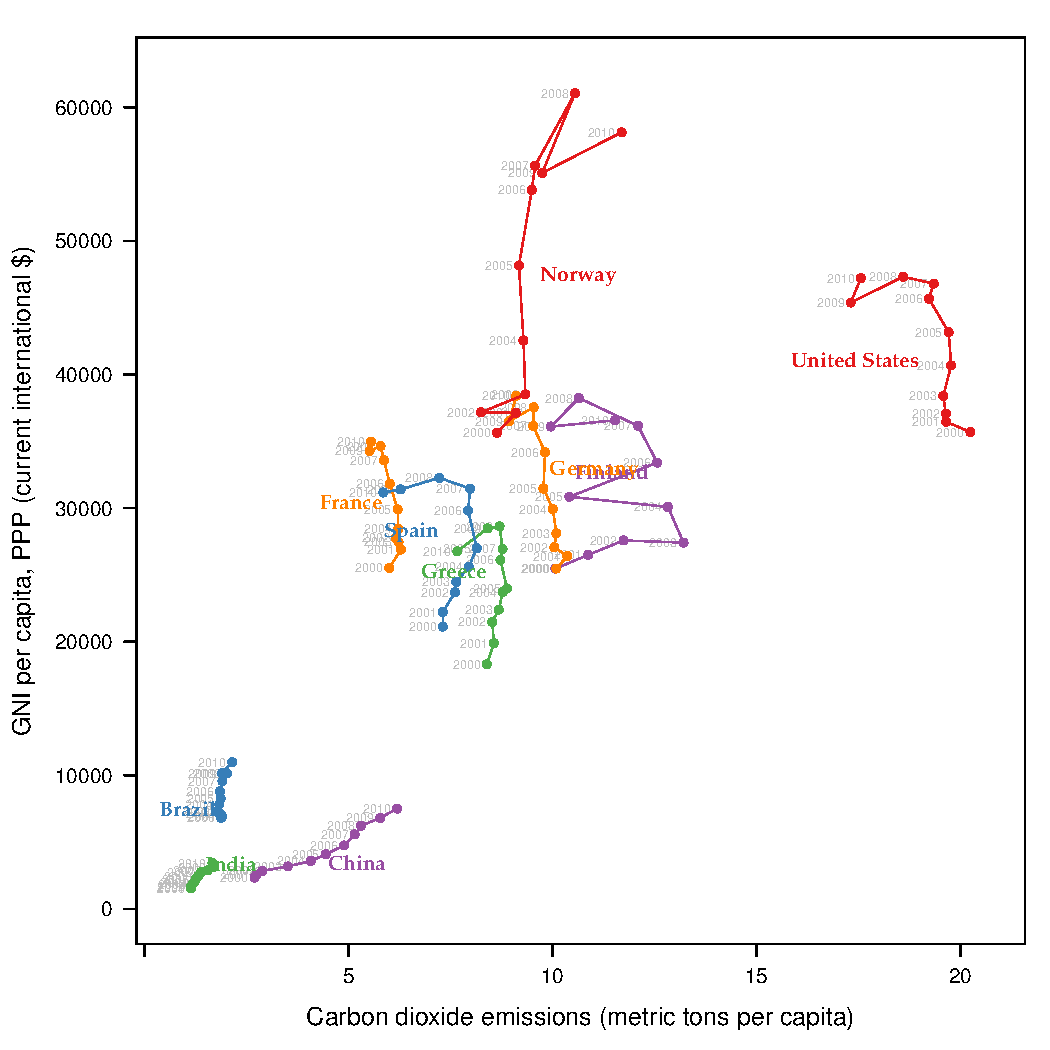
\includegraphics[width=.9\linewidth]{figs/CO2_capita.pdf}
\caption{\label{fig:CO2_GNI_glayer}$CO_2$ emissions versus GNI per capita. Labels are placed with \texttt{panel.text}.}
\end{figure}

This simple solution cannot solve the overlapping between labels
and lines. The package \texttt{directlabels} includes a wide repertory of
positioning methods to cope with this problem. The main function,
\texttt{direct.label}, is able to determine a suitable method for each
plot, although the user can choose a different method from the
collection or even define a custom method. For the \texttt{pCO2.capita}
object I have obtained the best results with \texttt{extreme.grid}.

\index{Packages!directlabels@\texttt{directlabels}}
\index{direct.label@\texttt{direct.label}}

\lstset{language=R}
\begin{lstlisting}
library(directlabels)
direct.label(pCO2.capita, method='extreme.grid')
\end{lstlisting}

\begin{figure}[htb]
\centering
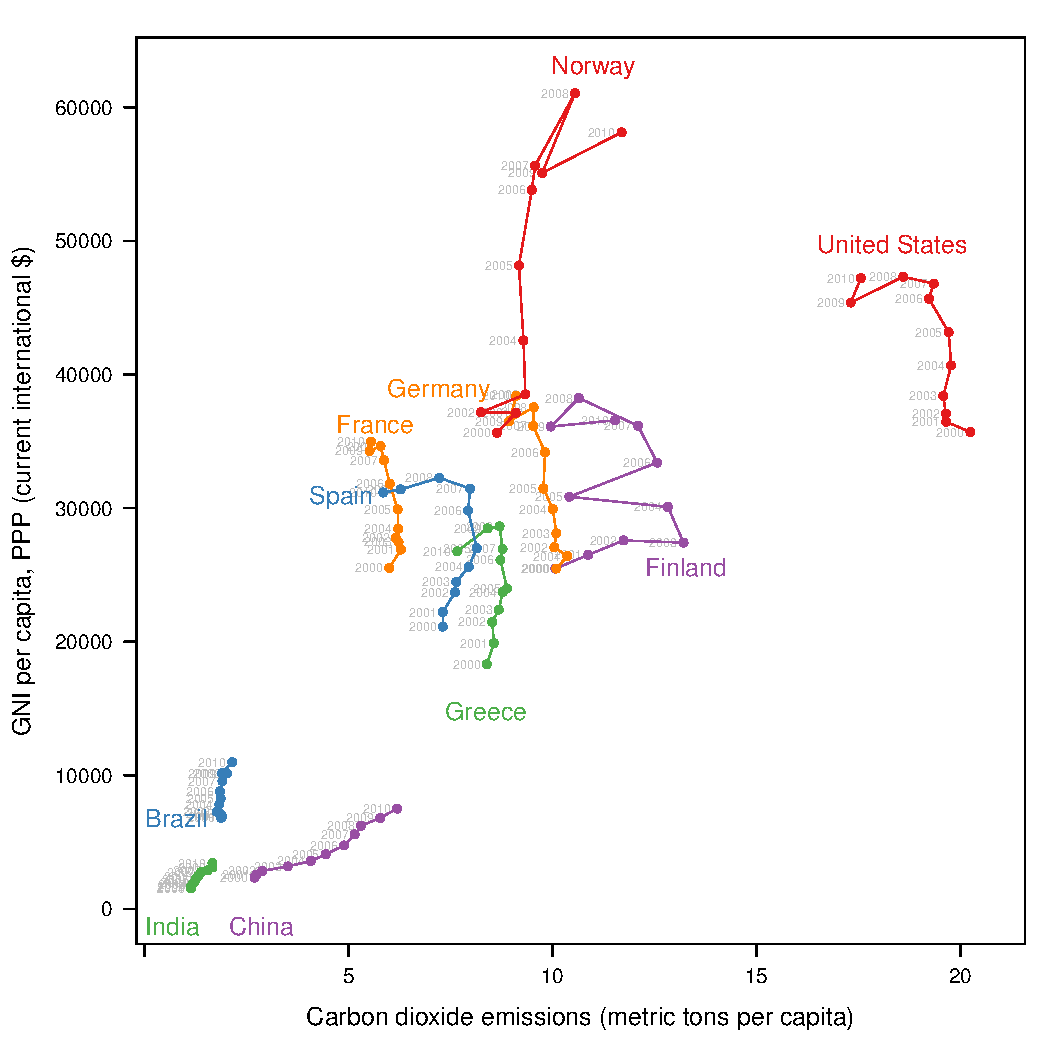
\includegraphics[width=.9\linewidth]{figs/CO2_capitaDL.pdf}
\caption{$CO_2$ emissions versus GNI per capita. Labels are}
\end{figure}
\subsection{Bubbles}
\label{sec-1-4}



\lstset{language=R}
\begin{lstlisting}
library(classInt)
z <- CO2data$CO2.PPP
intervals <- classIntervals(z, n=7, style='fisher')
nInt <- length(intervals$brks) - 1

idx <- findCols(intervals)

op <- options(digits=2)
tab <- classInt:::tableClassIntervals(cols = idx, brks = intervals$brks,
                                      under = "under", over = "over", between = "-", 
                                      cutlabels = TRUE,
                                      intervalClosure = "left",
                                      dataPrecision = NULL)
options(op)

size <- c(0.3, 2)
pwr.size <- 1
rval <- seq(1, 0, length=nInt)
cex.key <- size[2] - diff(size)*rval^pwr.size 
CO2data$cexPoints <- cex.key[idx]

key <- list(space='right',
            title='CO2.PPP', cex.title=1,
            text=list(labels=names(tab), cex=0.85),
            points=list(col='black', pch=19, cex=cex.key, alpha=0.7))
\end{lstlisting}


\lstset{language=R}
\begin{lstlisting}
xyplot(GNI.capita~CO2.capita|Year, data=CO2data,
       groups=Country.Name, key=key, alpha=0.7,
       strip=strip.custom(strip.levels=c(TRUE, TRUE)),
       panel=function(x, y, cex.values,..., subscripts, groups){
         panel.text(x, y, ...,
                    labels=groups[subscripts],
                    col=palOrdered[groups[subscripts]],
                    pos=3, cex=0.6)
         panel.points(x, y, col=palOrdered[groups[subscripts]],
                      cex=CO2data$cex[subscripts])
       })
\end{lstlisting}

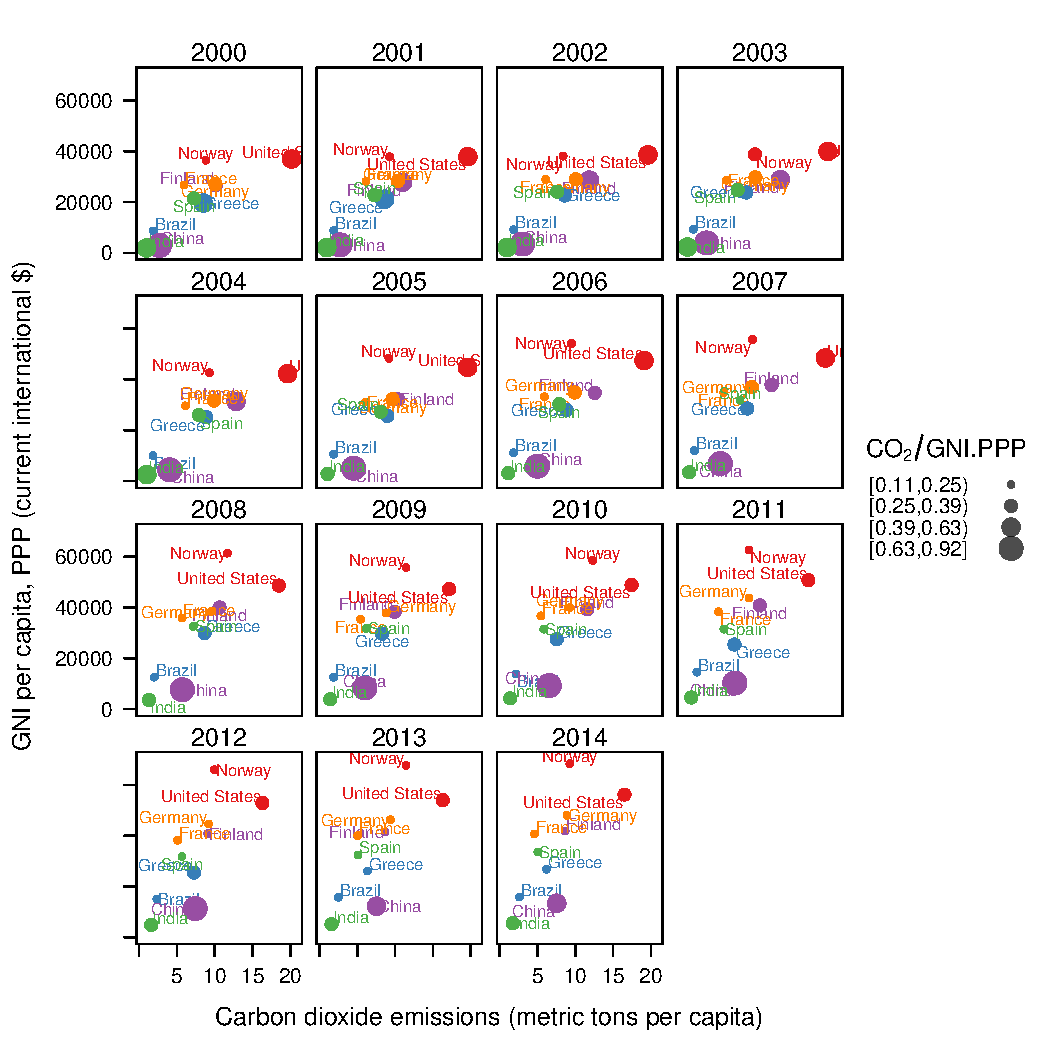
\includegraphics[width=.9\linewidth]{figs/CO2points.pdf}


\lstset{language=R}
\begin{lstlisting}
xyplot(GNI.capita~CO2.capita|Year, data=CO2data,
       groups=Country.Name, aspect=1,
       strip=strip.custom(strip.levels=c(TRUE, TRUE)),
       panel=function(x, y, ..., subscripts, groups) {
         color <- palOrdered[groups[subscripts]]
         radius <- CO2data$CO2.PPP[subscripts]
         grid.text(label=groups[subscripts],
                   unit(x, 'native'),
                   unit(y, 'native') + radius * unit(.15, 'inch'),
                   gp=gpar(col=color, cex=0.7))
         grid.circle(x, y, default.units='native',
                     r=radius * unit(.1, 'inch'),
                     gp=gpar(col=color,
                       fill=adjustcolor(color, alpha=.5),
                       lwd=1))
       })
\end{lstlisting}

\includegraphics[width=.9\linewidth]{figs/CO2bubbles.pdf}

    
\subsection{Animation}
\label{sec-1-5}



\lstset{language=R}
\begin{lstlisting}
library(gridSVG)

xyplot(GNI.capita ~ CO2.capita, data=CO2data,
       subset=Year==2000, groups=Country.Name,
       xlim=extendrange(CO2data$CO2.capita),
       ylim=extendrange(CO2data$GNI.capita),
       panel=function(x, y, ..., subscripts, groups) {
         color <- palOrdered[groups[subscripts]]
         radius <- CO2data$CO2.PPP[subscripts]
         grid.circle(x, y, default.units="native",
                     r=radius*unit(.25, "inch"),
                     name=trellis.grobname("points", type="panel"),
                     gp=gpar(col=color,
                       fill=adjustcolor(color, alpha=.5),
                       lwd=2))
         grid.text(label=groups[subscripts],
                   unit(x, 'native'),
                   unit(y, 'native') + radius*unit(.4, 'inch'),
                   name=trellis.grobname('labels', type='panel'),
                   gp=gpar(col=color, cex=0.7))
       })

nCountries <- nlevels(CO2data$Country.Name)

x_points <- animUnit(unit(CO2data$CO2.capita, 'native'),
                     id=rep(1:14, 9))
y_points <- animUnit(unit(CO2data$GNI.capita, 'native'),
                     id=rep(1:14, 9))
y_labels <- animUnit(unit(CO2data$GNI.capita, 'native') + CO2data$CO2.PPP * unit(.4, 'inch'),
                     id=rep(1:14, 9))

size <- animUnit(CO2data$CO2.PPP * unit(.25, 'inch'),
                 id=rep(1:14, 9))

grid.animate(trellis.grobname("points", type="panel", row=1, col=1),
             duration=20,
             x=x_points,
             y=y_points,
             r=size,
             rep=TRUE)

grid.animate(trellis.grobname("labels", type="panel", row=1, col=1),
             duration=20,
             x=x_points,
             y=y_labels,
             rep=TRUE)

years <- unique(CO2data$Year)
visibility <- matrix("hidden", nrow=length(years), ncol=length(years))
diag(visibility) <- "visible"
yearText <- animateGrob(garnishGrob(textGrob(years, .9, .15,
                                             name="year",
                                             gp=gpar(cex=2, col="grey")),
                                    visibility="hidden"),
                        duration=20,
                        visibility=visibility,
                        rep=TRUE)
grid.draw(yearText)

gridToSVG("figs/bubbles.svg")
\end{lstlisting}


\lstset{language=R}
\begin{lstlisting}
library(googleVis)
pgvis <- gvisMotionChart(CO2data, idvar='Country.Name', timevar='Year')
\end{lstlisting}
